\documentclass{sig-alternate}

\usepackage{amsmath}
\usepackage{graphics}
\usepackage{graphicx}
\usepackage{subfigure}
\usepackage{color}
\usepackage{xspace}
\usepackage{url}
\usepackage[utf8]{inputenc}

% reviews
\newcommand{\todo}[1]        {\textcolor{red}{[TODO] #1}}
\newcommand{\keoma}[1]       {\textcolor{blue}{[Keoma] #1}}
\newcommand{\ana}[1]         {\textcolor{blue}{[Ana] #1}}
\newcommand{\diego}[1]       {\textcolor{blue}{[Diego] #1}}
\newcommand{\remy}[1]        {\textcolor{blue}{[Remy] #1}}
\newcommand{\xavi}[1]        {\textcolor{blue}{[Xavi] #1}}
\newcommand{\thomas}[1]      {\textcolor{blue}{[Thomas] #1}}

 % lorem
\newcommand{\lorem}          {\textcolor{green}{Lorem ipsum dolor sit amet, consectetur adipisicing elit, sed do eiusmod tempor incididunt ut labore et dolore magna aliqua. Ut enim ad minim veniam, quis nostrud exercitation ullamco laboris nisi ut aliquip ex ea commodo consequat. Duis aute irure dolor in reprehenderit in voluptate velit esse cillum dolore eu fugiat nulla pariatur. Excepteur sint occaecat cupidatat non proident, sunt in culpa qui officia deserunt mollit anim id est laborum.}}

% shortcuts
\newcommand{\smip}           {SmartMesh~IP\xspace}
\newcommand{\HRNEIGHBORS}    {{\tt HR\_NEIGHBORS}\xspace}
\newcommand{\HRDISCOVERED}   {{\tt HR\_DISCOVERED}\xspace}
\newcommand{\HRDEVICE}       {{\tt HR\_DEVICE}\xspace}
\newcommand{\pathcreate}     {{\tt path\_create}\xspace}
\newcommand{\pathdelete}     {{\tt path\_delete}\xspace}
\newcommand{\motecreate}     {{\tt mote\_create}\xspace}
\newcommand{\HRNEIGHBORSTOTALNUMBER}     {140,897}

\graphicspath{{figures/}}

\begin{document}
\title{(Not so) Intuitive Results from a Smart Agriculture\\Low-power Wireless Mesh Deployment}

\numberofauthors{6}
\author{
    \alignauthor Keoma~Brun-Laguna\\
        \affaddr{Inria, EVA team,\\ Paris, France}\\
        \email{keoma.brun@inria.fr}
    \alignauthor Ana~Laura~Diedrichs\\
        \affaddr{Universidad Tecnológica Nacional (UTN)\\Mendoza, Argentina}\\
        \email{ana.diedrichs@frm.utn.edu.ar}
    \alignauthor Diego~Dujovne\\
        \affaddr{Universidad Diego Portales}\\
        \affaddr{Santiago, Chile}\\
        \email{diego.dujovne@mail.udp.cl}
    \and
    \alignauthor R\'emy~L\'eone\\
        \affaddr{Inria, EVA team,\\ Paris, France}\\
        \email{remy.leone@inria.fr}
    \alignauthor Xavier~Vilajosana\\
        \affaddr{Univ. Oberta de Catalunya, Barcelona, Catalonia, Spain}\\
        \email{xvilajosana@uoc.edu}
    \alignauthor Thomas~Watteyne\\
        \affaddr{Inria, EVA team,\\ Paris, France}\\
        \email{thomas.watteyne@inria.fr}
}

\maketitle

\begin{abstract}
\lorem
\end{abstract}

%==============================================================================
\section{Introduction}
\label{sec:intro}

% the PEACH project

Low temperatures have a very harmful impact on peach production as in 2013, 85\% of the production in the Mendoza region (western Argentina) was lost because of frost.
In April 2016, three research teams from different countries joined to start the deployment of a frost events prediction system~\cite{watteyne16peach}.
The goal of this project is to be able to precisely predict frost events and consequently reduce the impact of frost on peach production.
Frost detection systems already exist but few are actually able to propose prediction.

% the architecture

Due to the heavy machinery used to exploit the peach production, using cables is not conceivable.
The deployed solution is composed of a low-power wireless sensor network and a back-end system to retrieve and visualize the data.
The wireless network is formed by \smip devices from the Linear Technology company and is in charge of measuring the orchard environment such as air temperature and relative humidity.
The system collects both sensor values and network statistics and provide a visual interface and an API to access the data minutes after it was measured in Argentina.

% the deployment

The low-power wireless network is composed of 18 nodes uniformly distributed between the peach trees and 3 nodes to link up the orchards nodes and the gateway~\ref{fig:map}.
The covered area is an orchard with 204 trees on a 50*100m surface.
Each network mote is placed inside a water-tight box that is fixed on a 4m pole~\ref{fig:orchard}.
At the time of writing, the project is on its first stage.
During this stage, the goal is to verify that the network fulfill its requirements and that all the sensor values and statistics are correctly collected.
The current location and environment of the temperature sensors do not reflect reality, we do not exploit that information in this paper.
During the second stage, we will introduce additional sensors such as air temperature at different high, air relative humidity, soil moisture and soil temperature.

%======== front-page figure, do not move
\begin{figure}
    \centering
    \includegraphics[width=\columnwidth]{orchard}
    \caption{The wireless motes deployed in an orchard in Mendoza, Argentina.}
    \label{fig:orchard}
\end{figure}

\begin{table}
\begin{center}
    \begin{tabular}{ | l | l | l | l | l |}
         \hline
         \tt{38-0f-66}     & \tt{60-05-78} &                   &               & 1 \\
         \tt{60-06-ec}     & \tt{60-05-ab} & \tt{60-02-4b}     & \tt{60-02-1b} & 2 \\
         \tt{60-05-5f}     & \tt{60-06-27} & \tt{60-05-69}     & \tt{60-01-f8} & 3 \\
         \tt{3f-fe-87}     & \tt{3f-fe-88} & \tt{60-06-0f}     & \tt{60-08-d5} & 4 \\
         \tt{30-60-ef}$^*$ & \tt{3f-f8-20} & \tt{58-32-36}$^*$ & \tt{60-03-82} & 5 \\
         \hline
           \multicolumn{1}{|c|}{1} & \multicolumn{1}{|c|}{2} & \multicolumn{1}{|c|}{3} & \multicolumn{1}{|c|}{4} &\\
         \hline
    \end{tabular}
    \caption{The MAC addresses of the motes inside the orchard (last 3 bytes). Refer to numbers displayed on the map. ($^*$) DC9018 node with external antenna.}
\end{center}
\end{table}

\begin{figure*}
    \centering
    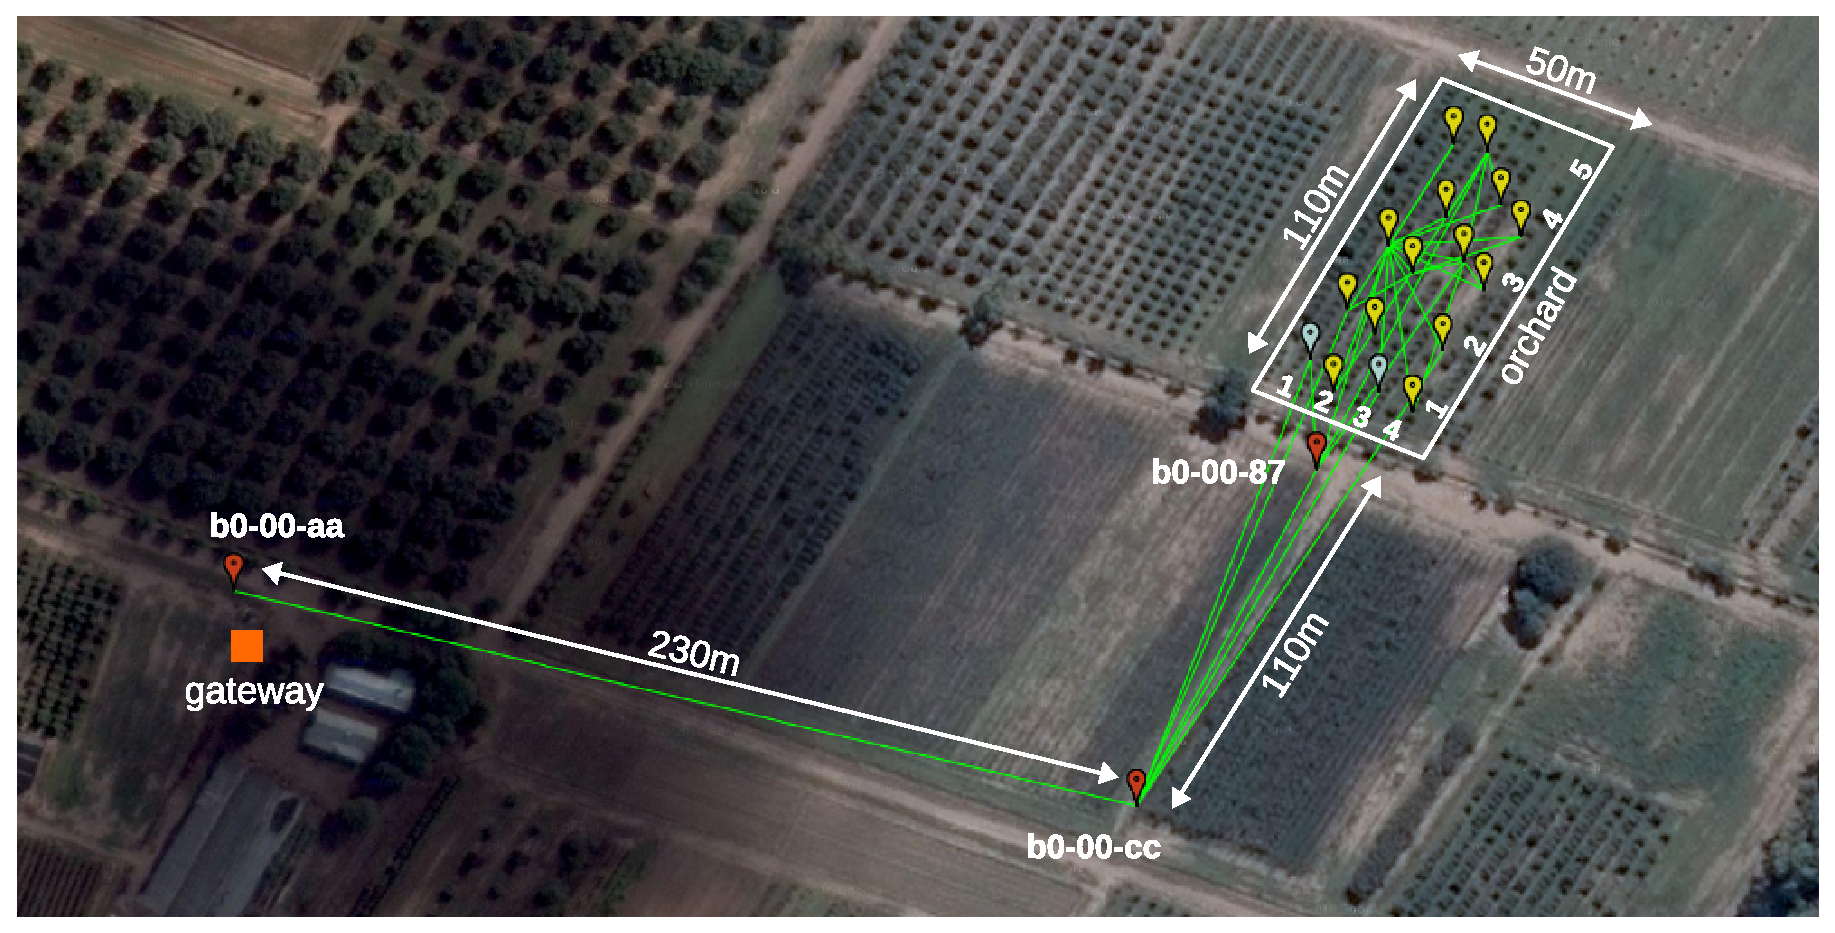
\includegraphics[width=\textwidth]{map_annotated}
    \caption{A map of the sensor deployed in the orchard near Mendoza, Argentina.}
    \label{fig:map}
\end{figure*}

% the hardware

We use four types of \smip devices to form the low-power wireless network.
The DC9018 with external antenna and the DC9003 with chip antenna are deployed inside the orchard.
Longe-range modes \keoma{@thomas: could you replace with exact name ?} are deployed outside the orchards to connect the network with the DC2274 device that is the gateway.

% the technology

The \smip motes are based on the IEEE 802.15.4e standard~\cite{std_ieee802154e} that includes a channel hopping mechanism to reduce the impact of multipath fading and external interferences.
Channel hopping exploit the frequency diversity to reduce the probability of interferences and improve link reliability.
This mechanism show good results in the Wireless Sensor Network (WSN) context~\cite{watteyne2010mitigating, watteyne2009reliability} and allows to achieve high reliability while saving energy.

% the data

Each mote produce a temperature value every 30 seconds and network statistics every 5~minutes.
In 4~months, we gathered more than 2M~temperature values, and more than 350K~network statistics.

% the goal of this paper

The goal of this paper is to present the first feedbacks we have from the 4-month-old project and the lessons we learned from analysing this WSN in real environment.
This paper makes the following contributions:
\begin{itemize}
    \item{We analyse network dynamic and show that channel hopping introduces high stability}
    \item{We analyse the link asymmetry and show that a link can be considered symmetrical in certain conditions}
\end{itemize}

% paper organisation

The remainder of this paper is organized as follows.
Section~\ref{sec:collected} describes what statistics we are collecting, and how much of it has been collected over 4 months.
Section~\ref{sec:intuitive} \todo{}.
Section~\ref{sec:notsointuitive} \todo{}.
Finally, Section~\ref{sec:conclusion} concludes this paper and discusses further improvements.

%==============================================================================
\section{Statistics Collected}
\label{sec:collected}

% where it is collected

The wireless network is deployed inside an orchard located in the country-side, around 45~km for Mendoza in Argentina.
Inside the field no other electronic device than the ones from the sensor network are present.
Local farmers work inside the field with heavy machinery approximately every 20 days for a period of one to two hours.
In the region the temperature can raise from $-9$~C in winter to +38~C in Summer.

% description health reports

Each device in the network produces both sensor data and network statistics.
Network statistics can be separated in \textbf{Events} and \textbf{Health Reports} messages.
The Events messages are non periodic information triggered when a node join/leave the network or when a link (layer 2) is created/deleted.
The Health Report (HR) message are sent periodically and provide counters and statistics to assess the overall network health.

% MOTE_CREATE

Each \smip is associated with an identifier called \textit{netId} that allows to have multiple networks cohabit in the same location.
When a mote wants to join a network, it listens for traffic and looks for devices that have the same \textit{netId} as itself.
Once it has identified the devices that share the same \textit{netid}, the node selects the best parent to send its joining request to.
The joining request will trigger a security handshake mechanism and produce a \motecreate event message.
This message contains the association between the newly-joined device's MAC address and a \textit{moteId} that is used for future communications.

% PATH_CREATE PATH_DELETE

To communicate with its neighbors, each devices creates `paths'.
In this paper, we use the word `path' and `link' interchangeably to designate a layer 2 resource reservation and its associated metrics (e.g signal strength, delivery ratio...).
When two nodes reserve resources to communicate with each others, a \pathcreate event message is produced.
When the nodes disallocate those resources, a \pathdelete is produced.

% HR_NEIGHBORS

Each node with an associated path is considered as a neighbor.
When deploying a \smip network, there are strong recommendations to follow, the most important one is that each nodes must have at least three `good' neighbors.
A neighbor is considered as `good' when the path with it has a stability superior to a configurable value.
The stability is given by the Packet Delivery Ration (PDR), i.e the percentage of successfully transmitted messages over the total number of transmitted messages.
Each node maintains a list of neighbors and periodically send \HRNEIGHBORS messages to the network manager.
\HRNEIGHBORS messages contain the path information with each neighbor.

% HR_DISCOVERED

Each node also maintains a list of `discovered neighbors' that are potential neighbors that can be used in case of path quality degradation with existing neighbors.
In the same way as \HRNEIGHBORS, nodes send \HRDISCOVERED messages that give information about the node potential neighbors such as RSSI value with that neighbor.

% HR_DEVICE

The network devices also produce \HRDEVICE messages give information about the mote itself.
\HRDEVICE messages include information such as node current battery voltage, internal temperature, and total number of messages the node has send.
Each device sends one type of Health Report (i.e \HRNEIGHBORS, \HRDISCOVERED, \HRDEVICE) every 5~min making the complete set of Health Reports generated every 15~min.

% messages stats

During the 4-month period we gathered an important amount of network statistics, presented in Table.\ref{tab:msg_stats}.
Possibly due to power line failure at the network manager side, the network experienced some restarting.
For this reason, some of the analysis presented in the next sections are done in shorter period of time.
As a side effect, this phenomenon allowed us to verify the network formation and joining process.

\begin{table}
    \centering
    \begin{tabular}{|l|r|}
        \hline
        \multicolumn{1}{|c|}{type} & \multicolumn{1}{|c|}{number} \\ \hline
        \hline
        \motecreate     &     133 \\ \hline
        \pathcreate     &   4,098 \\ \hline
        \pathdelete     &   3,653 \\ \hline
        \HRDEVICE       & 132,758 \\ \hline
        \HRNEIGHBORS    & \HRNEIGHBORSTOTALNUMBER \\ \hline
        \HRDISCOVERED   &  87,737 \\ \hline
    \end{tabular}
    \caption{The number of statistics collected over 4~months of network operation.}
    \label{tab:msg_stats}
\end{table}

%==============================================================================
\section{Intuitive Results}
\label{sec:intuitive}

\lorem

%------------------------------------------------------------------------------
\subsection{RSSI vs Distance}
\label{sec:rssi_distance}

From the Friis' transmission equation, we know that RSSI can be stated as function of distance.
To verify that our dataset corresponds to that equation we plot the RSSI over the distance (log-scale) of the data collected between the 18th of May to the 6th of June (19 days) in Fig.\ref{fig:pister_hack}.
We observe that all the values are located between the Friis' transmission equation and a -40dB shift.

\lorem

\begin{figure}
    \centering
    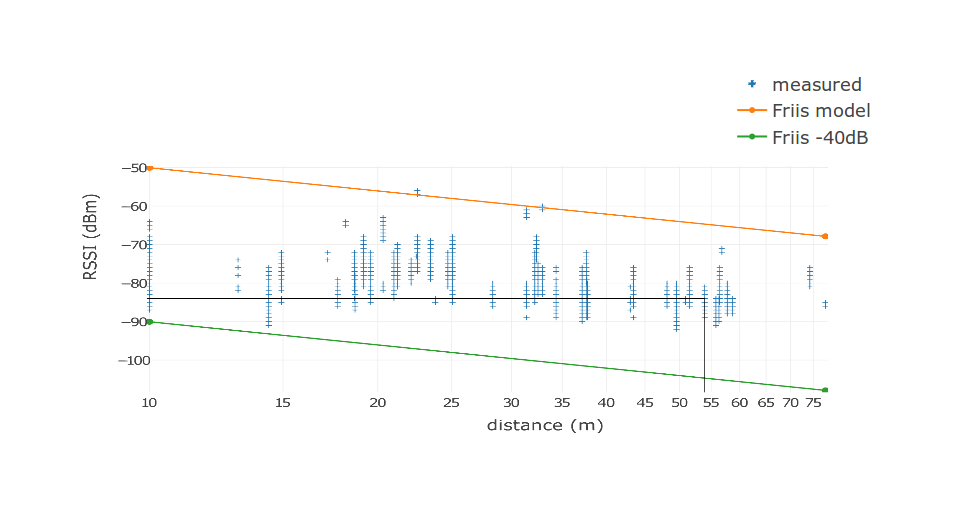
\includegraphics[width=\columnwidth]{pister_hack}
    \caption{All the measures are located between the Friis equation and a -40dB shift.}
    \label{fig:pister_hack}
\end{figure}

%------------------------------------------------------------------------------
\subsection{Wireless Waterfall}

% sample presentation

Due to the inherent physical unreliability of the radio medium, it is impossible to know if a future transmission will be successful or not.
The Packet Delivery Ratio (PDR) is the proportion of successful transmissions over the total number of transmissions.
Over a period of 4 months, \HRNEIGHBORSTOTALNUMBER \HRNEIGHBORS messages were collected.
Nodes maintain a list of potential neighbors with which they do not communicate with.
We removed the portion of neighbors with no transmission (237,252 messages) and kept only the DC9003 motes, resulting into a total of 125,103 messages (approx. 27\% from the total number of \HRNEIGHBORS).

% Waterfall

In Fig.\ref{fig:waterfall}, we show the so-called \textit{waterfall plot}, displaying the RSSI values against PDR values over the 4-months period.
A clear threshold appears when the RSSI values go below -85~dBm.
For RSSI values above that threshold, the PDR drastically decreases implying retransmission.
When the RSSI values are below that threshold, PDR values remain near 100\%, inducing successful transmissions.
The device manufacturer documentation~\cite{smip_app_note} indicates that a path is considered as "bad" when:

\begin{itemize}
  \item RSSI is above -80dBm and PDR < 50\%
  \item RSSI is above -70dBm and PDR < 70\%
\end{itemize}

% interferences

A waterfall plot either shifted right with very few path below -70dBm or with non-constantly decreasing curve would be an example of interference-prone environment.
As Fig.\ref{fig:waterfall} shows, devices do not have issues when communicating with links that have a low RSSI.
It means that high interferences are not present on the network.
This is confirmed by the large distance with other radio-communicating devices due to the location of the orchard.

\begin{figure}
    \centering
    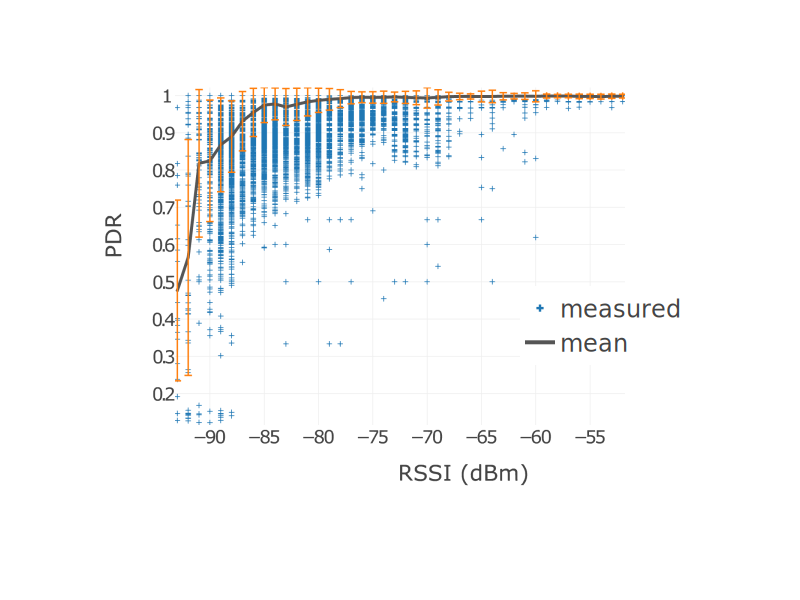
\includegraphics[width=\columnwidth]{waterfall}
    \caption{
        The PDR/RSSI waterfall.
        Links with low RSSI present good PDR showing the low interferences in the network.
    }
    \label{fig:waterfall}
\end{figure}

%------------------------------------------------------------------------------
\subsection{End-to-End Reliability}
\label{sec:net_reliability}

% steady state results

Table~\ref{tab:net_stats} presents the statistics from the last time the network restarted (i.e 10 days).
The results correspond to the ones presented in the project presentation paper~\cite{watteyne16peach} as stated:
``After approx. 24~hours of operation, a \smip network reaches steady state"".

All the 693,844 messages produced by the sensor network were received by the network gateway.
The stability, i.e the average PDR over the different links, increased of 2\%.
The latency, i.e the averaged time a message travel inside the network, lowered from 700~ms to 800~ms.

\begin{table}
    \begin{tabular}{|l|l|}
        \hline
        reliability & 100\% (Arrived/Lost:   693844/0)\\ \hline
        stability   & 95\% (Transmit/Fails: 4405569/258778)\\ \hline
        latency     & 700~msec\\
        \hline
    \end{tabular}
    \caption{The overall network statistic over the last 10 days.}
    \label{tab:net_stats}
\end{table}

%------------------------------------------------------------------------------
\subsection{Network Lifetime}
\label{sec:charge}

% description

Each device is powered by a pair of AA battery (Energizer L-91) with a charge of approximately 2821mAh.
The charge is measured by a built-in sensor inside the \smip board. \keoma{@thomas: could you give me more details?}

% results

Fig.\ref{tab:stats_charge} shows the device charge statistics over a 4-month period.
Every node is crucial in this application as each mode is connected to multiple sensors and represents one part of the orchard that could be prone to frost.
We thus consider the network lifetime as the time when the first node runs out of battery.
The node with the minimal amount of days left is node {\tt b0-00-cc} , that is one of the long-range node that is use to link up the orchard motes to the network gateway.
It is logical that this node spend more energy than the others as all the traffic passes through it, see Fig.~\ref{fig:map}.
Node {\tt b0-00-cc} has 1218 days left, that is above 3 years lifetime.
The node with the maximal amount of days left is node {\tt 60-02-4b}.
From~Fig.\ref{fig:map}, we can see that the node has no child and thus, do not retransmit any data from its neighbors.
There is a difference of 3513 days between the minimal and maximal lifetime.

\begin{table}
  \begin{tabular}{|c|c|r|}
     \hline
     MAC address    & charge consumed           &   lifetime \\
     \hline
     \tt{30-60-ef}  & 227,847~C (2.2\% battery) & 10.8~years \\
     \tt{38-0f-66}  & 252,356~C (2.5\% battery) &  9.8~years \\
     \tt{3f-f8-20}  & 291,312~C (2.9\% battery) &  8.4~years \\
     \tt{3f-fe-87}  & 392,606~C (3.9\% battery) &  6.3~years \\
     \tt{3f-fe-88}  & 458,459~C (4.5\% battery) &  5.3~years \\
     \tt{58-32-36}  & 327,634~C (3.2\% battery) &  7.5~years \\
     \tt{60-01-f8}  & 252,454~C (2.5\% battery) &  9.8~years \\
     \tt{60-02-1b}  & 222,253~C (2.2\% battery) & 10.1~years \\
     \tt{60-02-4b}  & 146,068~C (1.4\% battery) & 16.8~years \\
     \tt{60-03-82}  & 494,841~C (4.9\% battery) &  5.0~years \\
     \tt{60-05-5f}  & 274,502~C (2.7\% battery) &  9.0~years \\
     \tt{60-05-69}  & 437,136~C (4.3\% battery) &  5.7~years \\
     \tt{60-05-78}  & 304,145~C (3.0\% battery) &  8.1~years \\
     \tt{60-05-ab}  & 284,764~C (2.8\% battery) &  8.7~years \\
     \tt{60-06-27}  & 321,879~C (3.2\% battery) &  7.7~years \\
     \tt{60-08-d5}  & 263,120~C (2.6\% battery) &  9.3~years \\
     \tt{b0-00-87}  & 199,626~C (2.0\% battery) & 12.3~years \\
     \tt{b0-00-aa}  & 544,439~C (5.4\% battery) &  4.5~years \\
     \tt{b0-00-cc}  & 567,232~C (5.6\% battery) &  4.3~years \\
     \hline
  \end{tabular}
  \caption{The charge statistics.}
  \label{tab:stats_charge}
\end{table}

%==============================================================================
\section{Not so Intuitive Results}
\label{sec:notsointuitive}

\lorem

%------------------------------------------------------------------------------
\subsection{Link (A)Symmetry}
\label{sec:symmetry}

% RSSI expectations

The RSSI values can be retrieved from both active neighbors and discovered neighbors Health Reports, thus every 15~min for each pair of device.
Those RSSI values are averaged values over the 16 channels defined in the IEEE 802.15.4 standard~\cite{std_ieee802154_2011}.
In the rest of that paper we will use RSSI to denote the average RSSI over the 16 channels.

% environment

The peach orchard is located in a rural area that is not exposed to high traffic on the ISM band so we do not expect important external interferences.
Heavy machinery is used inside the orchard by farmers approximately every 20 days and during a period of one to two hours.
Those movements could create internal interferences such as multipath fading.

% symmetry analysis

A common assumption is to assume that a layer 2 link between two identical wireless nodes is asymmetrical.
We looked at the links statistics between the 18th of June and the 4th of July (16 days) and analysed the difference between the RSSI values.
The sample contains 411132 \HRNEIGHBORS messages and concerns 14 nodes with the same hardware (DC9003).
During that period, 21 different bidirectional links are active with at least 250 transmissions for each link.
For each of those links, we compute the RSSI difference between the two directions of the link (i.e from A to B and from B to A) and present the results in Fig.~\ref{fig:tab_symmetry}).
The very low RSSI difference shows that the links are very symmetrical.
Note that the RSSI is an averaged value over the different channels.

\begin{figure}
    \centering
    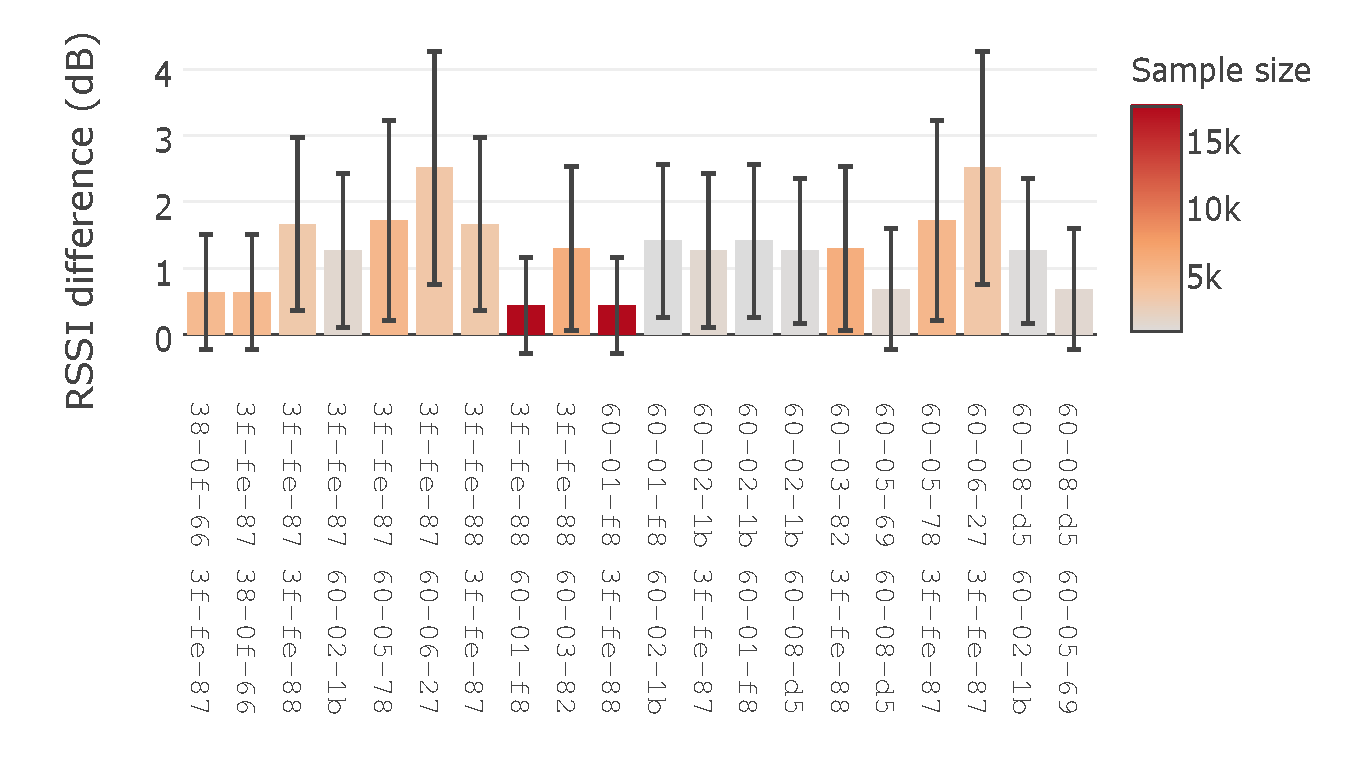
\includegraphics[width=\columnwidth]{sym_plot}
    \caption{The different active links between 2016-06-18 and 2016-06-25.}
    \label{fig:tab_symmetry}
\end{figure}

%------------------------------------------------------------------------------
\subsection{Network Stability}
\label{sec:net_stability}

% description

The nodes in the network form a Destination Oriented Direct Acyclic Graph (DODAG) oriented toward the gateway (i.e the DAG root).
Each node maintains a list of neighbors, with which they communicate or not, and dynamically change their routes depending on link quality. \keoma{@thomas:is it true ? or they use other metrics ?}
When reliability is high the network topology stay stable and the nodes use the same neighbors.
When the reliability decreases, nodes select other neighbors, making the network graph to change.
Instability in the network increases the signaling traffic to reconstruct the routes and introduce more bandwidth and energy consumption.

% results

To study the network stability we use the \pathdelete and \pathcreate event messages.
Those messages are sent every time a path with a neighbor is deleted or created responsively.
Here a path denotes a layer 4 association between two nodes.
Fig.\ref{fig:net_churn} shows the number of events message per hour as well as the total number of links per hour over a two-weeks period.
We can see that the number of links stay close to 35 for the entire period of time.
The number of \pathcreate and \pathdelete is also kept low.

\begin{figure}
    \centering
    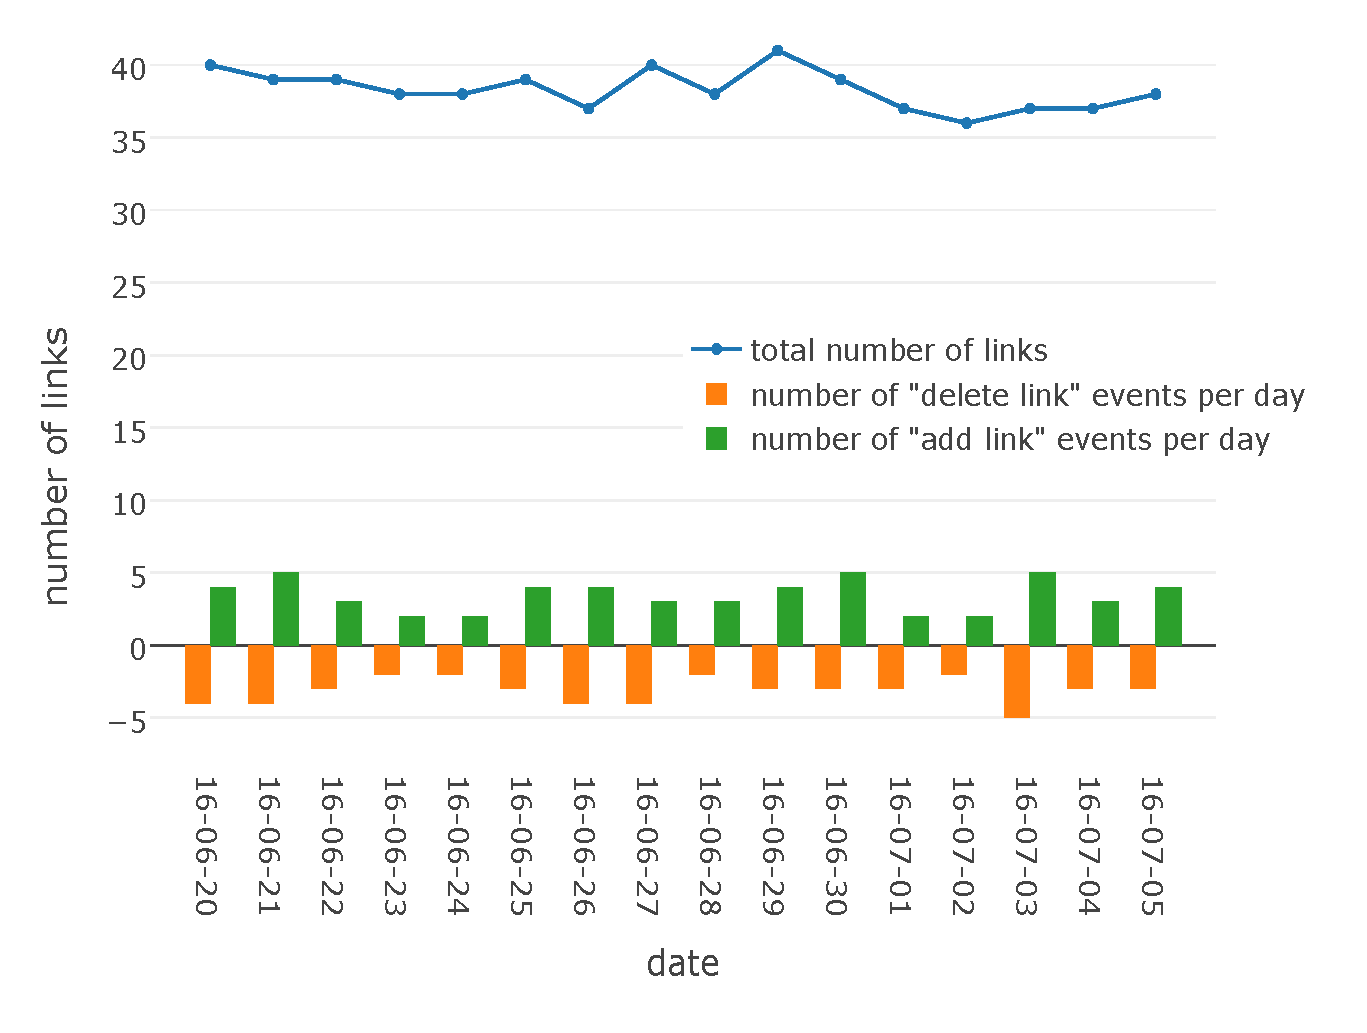
\includegraphics[width=\columnwidth]{net_churn}
    \caption{Network churn.}
    \label{fig:net_churn}
\end{figure}

%==============================================================================
\section{Conclusion}
\label{sec:conclusion}

% conclusion

\lorem

%==============================================================================

\bibliographystyle{abbrv}
\bibliography{brun16intuitive}

\end{document}
